\section{Insights} \label{sec:insights}
%
Since the main component of this project consists of learning the framework GraphX, we list some insights and what we have learned whiling exploring it.
%
\subsection{Advantages of GraphX}
%
\begin{figure}[t]
	\centering
	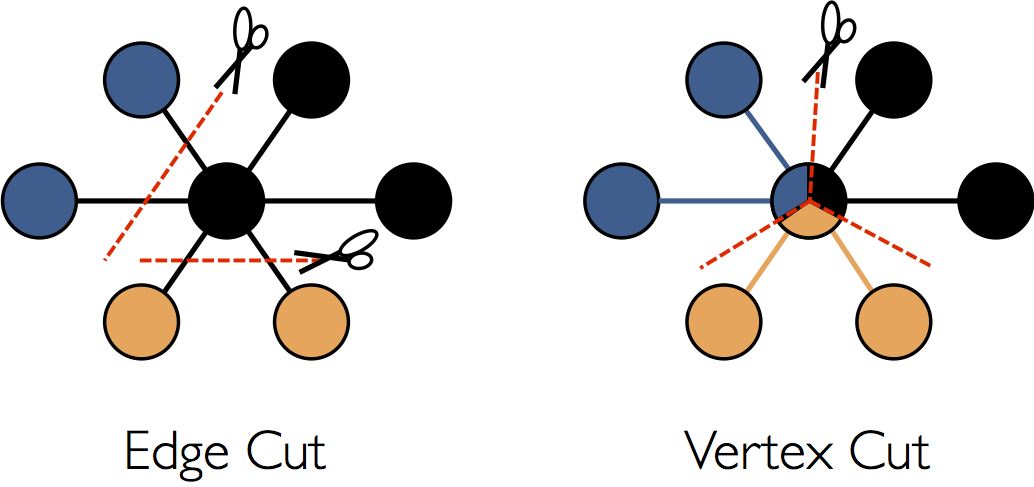
\includegraphics[width=0.7\linewidth]{edge_cut_vs_vertex_cut.png}
	\caption{Edge-based partitioning VS Vertex-based partitioning.}
	\label{fig:edgecut}
\end{figure}

Since GraphX is built on top of Spark, it adopts a lot of advantages from Spark.
%
One of the biggest advantages of GraphX is the easiness of implementation.
%
As the purpose of this project is to learn the framework, we choose not to use the PageRank function provided by GraphX.
%
Instead, we implement the PageRank algorithm by ourselves using Pregel API in GraphX.
%
However, the setup in order to initiate the execution of PageRank using Pregel only takes approximately 20 lines of code to complete.
%
Then, GraphX handles everything else for us, including fault-tolerance, concurrency control, etc..
%

There is one significant difference between the implementation of Pregel API in GraphX and standard Pregel implementation.
%
The Pregel API in GraphX only allows sending messages to the neighbors, whereas standard Pregel implementation can send messages to any vertex in the graph.
%
Although this sounds like a disadvantage, this "limitation" helps GraphX improve the efficiency.
%
Since in GraphX a graph is an extension of RDD, a graph dataset would be distributed across multiple machines.
%
Intuitively, we could partition a graph based on the vertices(Figure \ref{fig:edgecut}(a))\cite{Gonzalez:2014:GGP:2685048.2685096}, for example, by hashing vertex IDs. 
%
However, this would cause large communication overhead as a lot of messages need to be sent to across machines, which becomes a bottleneck of the computation.
%
Instead, GraphX handles graph partitioning in a edge-based manner (Figure \ref{fig:edgecut}(b)).
%
Edges are partitioned onto different machines and vertices are allowed to span on multiple machines.
%
This way, with the "limitation" that messages can only be sent to direct neighbors, we can partition the graph in a way that the communication overhead is very small.
%

\begin{table*}[ht]
	\centering
	\begin{tabular}{lccp{6.5cm}c}
		\toprule
		\textbf{Keywords}	& \textbf{Inverse count} 	& \textbf{Rank distance} 	&\textbf{Top one title} &\textbf{Top one citation}\\ \midrule
		Machine Learning	& 8					& 1.75			&Support-Vector Networks &33820\\
		Cryptography Security& 5					& 1.125			&State of the Art in Ultra-Low Power Public Key Cryptography for Wireless Sensor Networks &268 \\
		Distributed System	& 8					& 1.75			&Distributed Systems: Principles and Paradigms & 4038\\
		Deep Learning		& 11					& 2.25			&Deep learning via semi-supervised embedding &610\\
		Computer Vision 	& 8					& 1.5				&OpenVIDIA: parallel GPU computer vision & 281\\
		\bottomrule
	\end{tabular}
	\vspace{3mm}
	\caption{Results for selected keywords recommendation. }
	\label{res:keywordall}
\end{table*}

\begin{table*}[ht]
	\centering
	\begin{tabular}{lp{12cm}cc}
		\textbf{Keywords}	& Machine Learning \\ \hline
		\toprule
		\textbf{Rank}		& \textbf{Paper Title} 		& \textbf{Citation} 	&\textbf{Publish year}\\ \midrule
		1				&Support-Vector Networks 	&33820 &1995\\
		2				&Learning with Kernels: Support Vector Machines, Regularization, Optimization, and Beyond &10802&2001\\
		3				&Machine learning in automated text categorization &9095&2002\\
		4				&Application of argument based machine learning to law &3&2005\\
		5				&Data Mining: Practical Machine Learning Tools and Techniques&35014&2004\\
		6				&Very Simple Classification Rules Perform Well on Most Commonly Used Datasets&2060&1993\\
		7				&Investigating statistical machine learning as a tool for software development &59&2008\\
		8				&Machine Learning for User Modeling & 474&2001\\
		\bottomrule
	\end{tabular}
	\vspace{3mm}
	\caption{An example for keywords recommendation. }
	\label{res:keywordexp}
\end{table*}

\subsection{Disadvantages of GraphX}
%
While implementing algorithms in GraphX, we have also found some disadvantages of the framework.
%
First, we are not allowed to have different initial messages of Pregel API in GraphX for different types of vertices.
%
This has made the design of our pattern finding algorithm more challenging as we need to think of an initial message that would not mess up the attribute of any vertex.
%
The flexbility of initial messages may ease the implementation in some cases.
%
Secondly, since GraphX uses Pregel API, which is a synchronous model, the framework may not be the best fit for some algorithms, especially in machine learning and/or data mining.
%
In a synchronous model like Pregel, every vertex executes the same iteration.
%
That is, in the case that some of the vertices need more time to finish their vertex programs than the others, the entire computation is blocked.
%
An asynchronous model can make the computation a lot fast as the most recent information is being used, as opposed to previous iteration.
%
